\documentclass[a4paper,12pt]{article}
\usepackage[utf8]{inputenc}
\usepackage[english]{babel}
\usepackage{graphicx}
\usepackage{amsmath}
\usepackage{amssymb}
\usepackage{hyperref}
\usepackage{geometry}
\usepackage{tabularx}
\usepackage{float}
\usepackage[backend=biber, style=numeric, sorting=none]{biblatex}
\usepackage{booktabs}
\usepackage{colortbl}
\usepackage{xcolor}
\usepackage{caption} % For customising captions



% Set the caption font size
\captionsetup{font=small}


\addbibresource{references.bib}

\geometry{a4paper, left=25mm, right=25mm, top=25mm, bottom=25mm}
\title{Project 2: Reinforcement Learning - Q-Learning and Deep Q-Learning}

\author{Alexander Svarfdal Gudmundsson and Jan Babin}
\date{\today}

\begin{document}

\maketitle

\begin{center}  
    
\includegraphics[width=0.6\textwidth]{HR_logo.jpg}
\end{center}

\clearpage

\tableofcontents

\clearpage

\section{Introduction}
The main objective of this project is to apply Q-learning and Deep Q-learning to train an agent in a Flappy Bird game. 
The reason why reinforcement learning is applicable is because we can make an agent run in an simulated environment, 
even making the agent play at a much faster pace than in real time. 
In Flappy Bird you as the player play as a bird in a 2d environment where there are two pipes that appear to the right of the screen one coming from above and one coming from the top, 
with each consecutive frame the pipes move closer to the bird, and your task is to locate the bird by flapping its wings to make it fit between these two pipes. 
Flappy Bird is an interesting game to take on because it has a good balance between simplicity and challenge. 
Q-learning algorithm uses a tabular structure to learn every single possible state of the game to then take the best possible action that it knows. 
The Deep-Q learning uses function approximation to estimate whats the best action depending on what state the game is in. 

\section{Problem Description}
We were tasked with finding a sweetspot for the policy so that it would be as good as possible while involving as 
little game simulations as
possible. For our problem, having unlimited training episodes should (at least for q-learning) result in convergence towards an agent 
that never dies in the game.
However, this is obviously not feasible in reality. Hence, looking for a good-enough solution is very much motivated by
how such problems would be tackled in the industry.

\section{Characterisation of the Environment}
The environment techniqually is \textit{continuous} since for example the velocity of the bird or the coordinates of its whereabouts
could be represented by float values. In practise, it is probably both \textit{discrete} and \textit{finite} as for the bird's position we can consider a 
integer grid of pixels and the velocity may only take values from a countable and finite set of float values. Furthermore, the agent
may only choose from two possible actions for every state: to flap or not to flap - that is the question.
\\
The game is largely deterministic, with the bird's movements being accurately predictable as well as the pipes' behaviour once they have
appeard.
However, there is obviously some \textit{stochasticity} involved in their generation: 
The location of newly spawned pipes is random. Still, one could argue
this does not make it stochastic from the agents point of view, but more about that in the following sections.
\\
FlappyBirds is an episodic game: An episode starts with the bird alive and ends once it dies. Starting another iteration is independent
of the last one.
For an agent, to make informed decisions a state of FlappyBirds should contain the position and velocity of the bird as well as the distance to
and the height of the next pipe.
Furthermore, the game can inherently be modelled as a Markovian process: Knowing the current state is sufficient to predict the (close) future
and choose the next move. That is, if we know the status of our bird and the position of the next pipe, an agent can be able
to maneuver without crashing, unknowing of previous pipes or ones that will come after. Knowing subsequent pipes is only 
interesting for training to evalue future rewards.


\section{Implementation of Q-Learning}
\subsection{State Representation and Action Space}

\noindent State variables that describe the current environment that the agent is in:
\begin{itemize}
    \item \textbf{player\_y}: The current vertical position of the bird
    \item \textbf{next\_pipe\_top\_y}: The horizontal position of the next top pipe
    \item \textbf{next\_pipe\_bottom\_y}: The horizontal position of the next bottom pipe
    \item \textbf{next\_pipe\_dist\_to\_player}: The horizontal distance from the next pipe to the bird
    \item \textbf{next\_next\_pipe\_top\_y}: The horizontal position of the top pipe after the next
    \item \textbf{next\_next\_pipe\_bottom\_y}: The horizontal position of the bottom pipe after the next
    \item \textbf{next\_next\_pipe\_dist\_to\_player}: The horizontal distance from the pipe to the bird after the next
    \item \textbf{player\_vel}: The current velocity of the bird
\end{itemize}

\noindent The actions that the agent can take:
\begin{itemize}
    \item \textbf{flap}: The agent can choose to flap the wings causing the bird to gain altitude
    \item \textbf{no-flap}: The agent can choose to not flap the wings causing the bird to lose altitude
\end{itemize}

\noindent For the Q-learning we opted to bin (discretise) the values so that the q-table would not be insanely big. We split the space of these attributes (except the velocity) evenly
into 15 intervals each, resulting in at most 64125 different states to consider (not all of those are reachable).

\subsection{Q-Learning Algorithm}
The core of Q-Learning is a table, that assigns a Q-value to each combination of state \(s\) and action \(a\). These values represent the expected future
rewards for taking that action from that state. Training equals to constantly modifying the table, updating the Q-values. When training, Q-Learning chooses in a state
the action that has the highest Q-value (\textit{exploitation}) or a random action (\textit{exploration}), as governed by a hyperparameter \(\epsilon\).
Then it observes the next state \(s'\) and reward \(r\) to update the Q-table:
$$
Q(s, a) \leftarrow Q(s, a) + \alpha \left[ r + \gamma \max_{a'} Q(s', a') - Q(s, a) \right]
$$

\section{Implementation of Deep Q-Learning}
\subsection{Model Setup}
Explain the structure of the neural network, including the input normalisation, hidden layers, output layer, and activation functions.
The action space is the same as above for the Q-learning one but the state representation is not binned in this case but instead normalised using min-max normalisation.
The description stated a nice starting point, using two networks with hidden layers, 100 neurons in the first layer and 10 in the second layer. 
These two networks will then be used in tandem to train the model.

\subsection{Deep Q-Learning Algorithm}
The algorithm uses the idea of Q-learning to determine Q-values for actions in state but it does not use a Q-table, it uses a deep neural network to approximate the Q-values.
The deep neural network is then called a Deep-Q-Network. 
The algorithm makes the use of a replay buffer that stores past observations, it breaks correlations and stabilises training by learning from many past experiences. 
The algorithm also makes use of a target network that gets replaced by the main network on a predefined interval, the traget network provides a stable Q-value to improve stability in training.
Furthermore the algorithm uses batch sized sample from the replay buffer to update the Q-network.


\section{Experimental Results and Analysis}
\subsection{Learning Curve Analysis}
We employed Learning Curve Analysis to compare Q-Learning and Deep Q-Learning. For this we incrementally trained the models
for blocks of 1000 episodes, ran the trained policy / model up to that point on the game and averaged the scores. We then
plotted these scores against the number of episodes to get an idea of how the quality of the policy develops over time / training
episodes.

\begin{figure}[H]
    \centering
    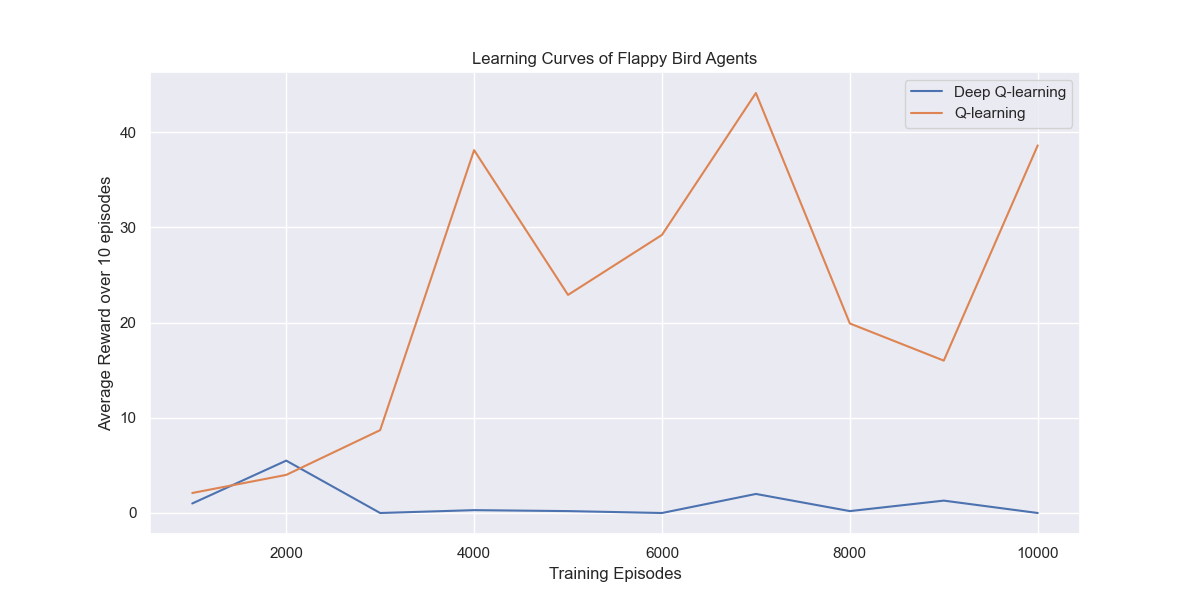
\includegraphics[width=\textwidth]{training_deepq_vs_q_avg10samples.png}
    \caption{Learning curves for Q-learning and Deep Q-learning agents in Flappy Bird. The average reward over 1 episode is plotted against the number of training episodes.}
    \label{fig:learning_curves}
\end{figure}

From this, one can safely assume that the Q-Learning agent will become better as the training amount increases. However,
for Deep Q-Learning the same could be expected but this is not indicidated by the plot. Assumingly, we would have to optimise the
hyperparameters further. We decided not to do that and stick to Q-Learning for hyperparameter optimisation, so as to cater to time constraints we had.
Q-Learning is quicker to train when only accessing CPU-power.

\subsection{Parameter Tuning}

\begin{itemize}
    \item \textbf{Discount rate}: Determines how far ahead we look into the future in terms of the rewards i.e. how farsighted or nearsighted our agent is
    \item \textbf{Learning rate}: Hyperparameter that controls how much value the agent treats our new information in contrast to the old Q-value in the table 
    \item \textbf{Greedy epsilon}: This controls how much we exploit vs explore, can be from 0 to 1, the higher the epsilon the more we explore 
\end{itemize}
For the hyperparameter tuning, we use random grid search to find the best combination of the parameters for the Deep Q-Learning agent. We randomly tried 20 different
hyperparameter combinations and trained each of the corresponding models on 2000 episodes.

\subsection{Best Performing Agent}
\begin{table}[h]
    \centering
    \caption{Best Hyperparameter Combination for Q-learning}
    \begin{tabular}{|c|c|}
        \hline
        Hyperparameter & Value \\
        \hline
        Discount Rate (\(\gamma\)) & 0.950 \\
        \hline
        Learning Rate (\(\alpha\)) & 0.096 \\
        \hline
        Exploration Rate (\(\epsilon\)) & 0.014 \\
        \hline
    \end{tabular}
    \label{tab:best_hyperparams}
\end{table}

The best combination of hyperparameters we could find is shown in Table \ref{tab:best_hyperparams}. We then initialised a 
new agent with these settings and also an agent with default settings and trained both for 3000 episodes. The tuned agent 
performed significantly better (see Figure \ref{fig:comparison.png}). After that, we trained our best agent for 10000 episodes, 
tracking the progress by plotting the learning curve as can be seen in Figure \ref{fig:learning_curve_best}.

\begin{figure}[H]
    \centering
    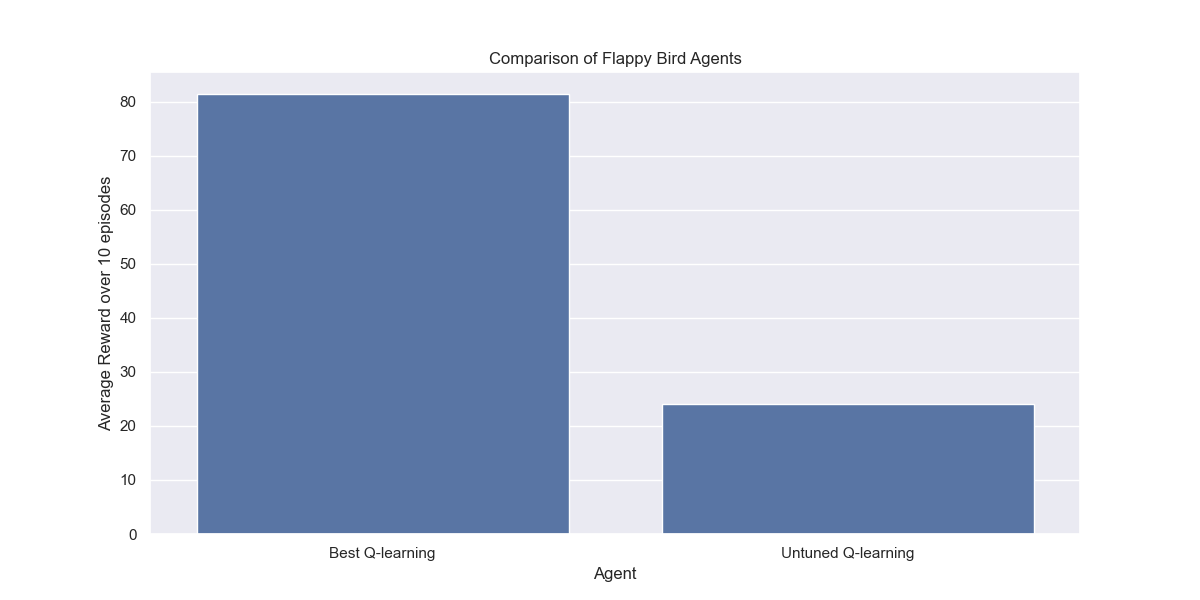
\includegraphics[width=\textwidth]{comparison.png}
    \caption{Comparison between average scores of 10 games between the tuned and the untuned agent.}
    \label{fig:comparison.png}
\end{figure}

\begin{figure}[H]
    \centering
    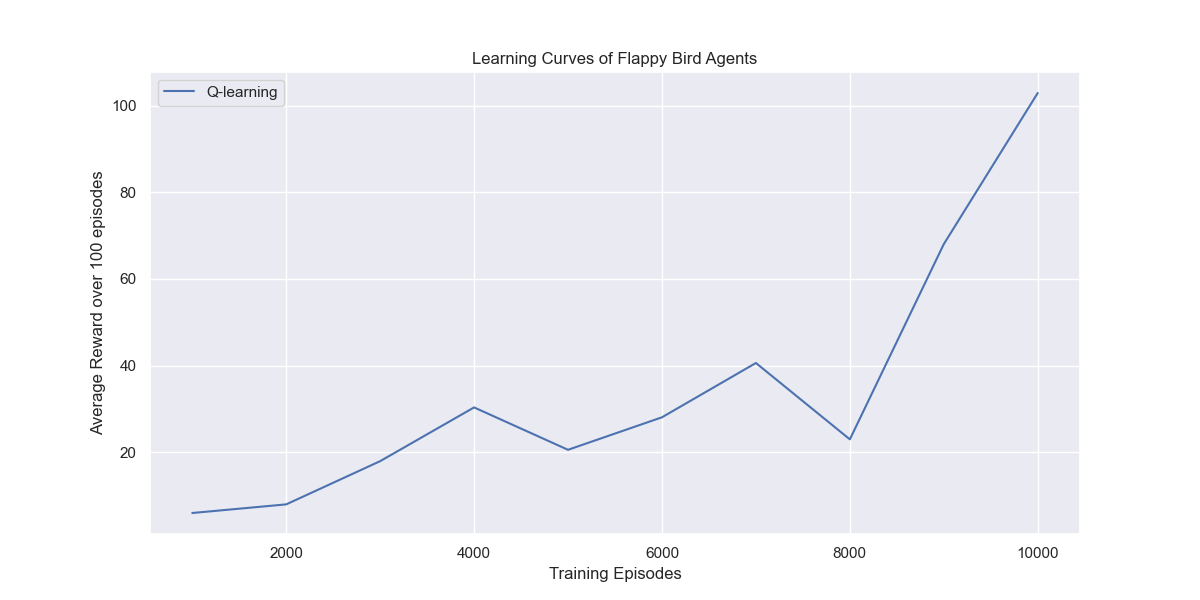
\includegraphics[width=\textwidth]{tuned_q_learning_10000.png}
    \caption{Learning curve of best tuned model on 10000 episodes.}
    \label{fig:learning_curve_best}
\end{figure}

\section{Conclusion and Future work}
Q-Learning turned out to be a robust method to find a reliable agent as was expected. Using 15 buckets for the state attributes is precise enough to
control the bird, so that it only dies in "unforeseen" states, that is, states that the agent had not encountered that often. We assume that our agent
will converge towards a perfect player of the game (i.e. bird never dies) as the number of episodes increase.
\\
The Achilles' heel of our solution is that the Deep Q-learning agent did not perform as well as we hoped, 
after certain amount of episodes it converged to be a worse agent, this pattern can be seen in figure \ref{fig:learning_curves}.
Due to this shortcoming the future work would consist of fixing this agent so it does not get worse over time. 
As figure \ref{fig:learning_curves} depicts the Deep Q-learning agent shows some improvement trianing on only 2000 episodes but then it plumits after 3000 episodes to a average reward over 1 episode of around 0. 
As of now we dont know the reason why, we tried to troublshooting this (possibly spent too much time on that) but with no luck. 


\begin{figure}[H]
    \centering
    
\includegraphics[width=0.5\textwidth]{ai_image.jpg}
    \caption{FlappyBirds in Machine Learning - Created by \href{https://gemini.google.com/}{Google Gemini}}
    \label{fig:gemini}
\end{figure}


\end{document}